\documentclass[]{beamer}
\usepackage[utf8]{inputenc}
\usepackage[T1]{fontenc}
\usepackage{default}
\usepackage[ngerman]{babel}

\usepackage{datetime}

%\usepackage{caption,subcaption}
\usepackage{natbib}

% \usepackage{overpic}
\usepackage{floatflt}
\usepackage{tikz}
\usepackage{pgf}
\usepackage{bm}

\usepackage{array}
\usepackage{booktabs}
\usepackage{enumerate}

\usepackage{amsmath}
\usepackage{listings}
\lstset{language=Python,numbers=left,escapeinside={[}{]}}

\usepackage{graphicx}

\usepackage{todonotes}
\presetkeys{todonotes}{inline,size=\tiny}{}

\makeatletter
\newenvironment{myitemize}{%
   \setlength{\topsep}{0pt}
   \setlength{\partopsep}{0pt}
   \renewcommand*{\@listi}{\leftmargin\leftmargini \parsep\z@ \topsep\z@ \itemsep\z@}
   \let\@listI\@listi
   \itemize
}{\enditemize}
\makeatother

\newcommand{\executeIfFileNewer}[3]{%
  \ifnum\pdfstrcmp{\pdffilemoddate{#1}}{\pdffilemoddate{#2}} > 0%
    \immediate\write18{#3}%
  \fi%
}

\graphicspath{{figures/pdf/},{figures/}}

\newcommand{\inputSVG} [2][]{%
  \executeIfFileNewer{figures/#2.svg}{figures/pdf/#2.pdf}{%
    inkscape -z -D --file=figures/#2.svg --export-pdf=figures/pdf/#2.pdf --export-latex --export-area-drawing}%
  #1%
  \input{figures/pdf/#2.pdf_tex}%
}

\newcommand\Wider[2][3em]{%
\makebox[\linewidth][c]{%
  \begin{minipage}{\dimexpr\textwidth+#1\relax}
  \raggedright#2
  \end{minipage}%
  }%
}

\usetheme{Antibes}
\usecolortheme{dolphin}

\setbeamercovered{transparent}
\beamertemplatenavigationsymbolsempty
\setbeamertemplate{footline}[frame number]

% \setbeamercolor{title}{fg=red!80!black,bg=red!20!white}

\usefonttheme[onlylarge]{structuresmallcapsserif}
\usefonttheme[onlysmall]{structurebold}

\title{Meine Privatsphäre im Internet}

\author[T. Bopst, S. Köhler]{Thomas Bopst, Steffen Köhler}
\newdateformat{writtenDate}{\THEDAY. \monthname[\THEMONTH]~\THEYEAR} % d. MONAT yyyy
\date{\writtenDate\formatdate{18}{12}{2014}\\[2em]

\includegraphics[width=0.3\textwidth]{figures/CC_by_4.png}}

\begin{document}
\bibliographystyle{apalike}

\frame{\titlepage}

\section*{Fragen}

\setbeamercovered{invisible}
\begin{frame}
  \frametitle{Fragen}

  \begin{itemize}
   \item Wer sorgt sich um die eigene Privatsphäre?
   \pause
   \item Hast du ein Problem damit, dass Andere deine Textnachrichten mitlesen?
   \pause
   \item Was für Maßnahmen unternehmt ihr um eure Textnachrichten zu schützen?
   \pause
   \item Wer würde seine Nachrichten gerne schützen, weiß jedoch nicht wie?
  \end{itemize}

\end{frame}



\frame{%
  \frametitle{Inhaltsverzeichnis}
  \tableofcontents
}

\section{Einleitung}

\begin{frame}
  \frametitle{Motivation}

  Ziele:
  \begin{itemize}
   \item Bewusstsein für Privatsphäre im digitalen Raum schaffen
   \item Möglichkeiten zum Schutz der Privatsphäre aufzeigen
  \end{itemize}

  \vspace{2ex}

  Was wir nicht wollen:
  \begin{itemize}
    \item Eine Musterlösung vorgeben!
    \item Missionieren
  \end{itemize}
\end{frame}


\section{Deine Spuren im Netz}

\begin{frame}
\frametitle{Was ist ein Cookie?}

\begin{itemize}
  \item Identifikationsnummer, die vom Anbieter vergeben wird
  \item Verwendet um BesucherInnen wiederzuerkennen
\note{Notwendig für Sessions}
  \item Werden im Web-Browser gespeichert
\note{IE, Firefox, Safari ...}
  \item Werden in der Regel nicht automatisch gelöscht
  \item $\rightarrow$ bspw. kein erneuter Login notwendig
\note{Google, Facebook, GMX, ...}
\end{itemize}

\end{frame}

\begin{frame}
\frametitle{Profilbildung im Netz}

\begin{itemize}
  \item Like (Facebook), +1 (Google), Tweet (Twitter), \dots
  \item Über Cookies mit persönlichem Profil verknüpfbar
\note{ggf. werden Daten an dritte weitergegeben (Versicherungen etc)}
\note{personalisierte Werbung}
\note{TODO Bild Hänsel und Gretel mit Cookiespur}
\end{itemize}

\end{frame}

\begin{frame}
  \frametitle{Wie schütze ich mich davor}
  \begin{itemize}
    \item Cookies löschen?
    \item Ghostery, etc.
   \note{Disconnect, TrackMeNot}
    \item Adblocker
    \item DuckDuckGo
   \note{Cookies von Werbeanbietern}
  \end{itemize}
\end{frame}


% Überleitung zu Instantmessaging, da ja noch viel schlimmer.

\section{Grundlagen Kryptographie}

\frame{%
  \frametitle{Inhaltsverzeichnis}
  \tableofcontents[currentsection]
}

\begin{frame}
  \frametitle{Übertragungsweg von Nachrichten}
  \center \inputSVG[\def\svgscale{0.25}]{Orange_blue_message_transportation_de}
  \begin{itemize}
    \item Nachrichten werden an Server geschickt
    \item von dort aus weiter an Empfänger geleitet
    \item $\rightarrow$ Jeder kann mitlesen
  \end{itemize}

  \note{Analogie: Brief/Postkarte mit Adresse}
\end{frame}

\begin{frame}
  Ende-zu-Ende Verschlüsselung
  \begin{center}
    \inputSVG[\def\svgscale{0.25}]{Orange_blue_message_end_to_end_de}
  \end{center}
  
  \frametitle{Transportwegverschlüsselung / Ende-zu-Ende Verschlüsselung}
  Transportwegverschlüsselung
  \begin{center}
    \inputSVG[\def\svgscale{0.25}]{Orange_blue_message_transportation_security_de}
  \end{center}
\end{frame}

\begin{frame}
  \frametitle{Transportweg- und Ende-zu-Ende Verschlüsselung}
  \begin{center}
    \inputSVG[\def\svgscale{0.25}]{Orange_blue_message_transportation_end2end_de}
  \end{center}
  \begin{itemize}
    \item Meta-Daten auf dem Transportweg geschützt
    \item Provider kann nicht mitlesen
  \end{itemize}
\end{frame}


\begin{frame}
  \frametitle{Symmetrische Verschlüsselung}
  \center \inputSVG[\def\svgscale{0.2}]{Orange_blue_symmetric_scheme_de}
  %\todo[inline]{Schaubild Verschlüsselung (symm)}
\end{frame}

\begin{frame}
  \frametitle{Probleme symmetrischer Verschlüsselung}
  \begin{itemize}
    \item Verteilung der Schlüssel
    \item Anzahl benötigter Schlüssel
    \begin{itemize}
      \item 2 Personen $\rightarrow$ 1 Schlüssel
      \item 3 Personen $\rightarrow$ 3 Schlüssel
      \pause
      \item 4 Personen $\rightarrow$ 6 Schlüssel
      \item 100 Personen $\rightarrow$ 4950 Schlüssel
      \item n Personen $\rightarrow$ $\frac{n^2-n)}{2}$ Schlüssel
    \end{itemize}
  \end{itemize}
\end{frame}

\begin{frame}
  \frametitle{Asymmetrische Verschlüsselung}
  \framesubtitle{Grundlagen}
  \begin{columns}[c]
    \begin{column}{0.5\textwidth}
      \center \inputSVG[\def\svgscale{0.2}]{Orange_blue_public_private_keygeneration_de}
    \end{column}
    \begin{column}{0.5\textwidth}
      \center \inputSVG[\def\svgscale{0.2}]{Orange_blue_public_key_cryptography_de}
    \end{column}
  \end{columns}
\end{frame}

\begin{frame}
  \frametitle{Asymmetrische Verschlüsselung}
  \framesubtitle{Schema}
  \center \inputSVG[\def\svgscale{0.2}]{Orange_blue_public_key_scheme_de}
\end{frame}

\section{Instant Messaging}

\frame{
  \frametitle{Inhaltsverzeichnis}
  \tableofcontents[currentsection]
}

\begin{frame}
  \frametitle{Open Source vs. Closed Source}
  \begin{definition}[Open Source]
   Programm mit öffentlich zugänglichem Quellcode \hfill \tiny [Duden]
  \end{definition}

  \begin{itemize}
   \item Programm kann von jedem geprüft werden
   \item Schwer Hintertüren einzubauen
   \item Notwenige Bedingung für prüfbar sichere Programme
   \item Open Source $\neq$ kostenlos
  \end{itemize}
\end{frame}

\begin{frame}
  \frametitle{Identitätsprüfung}
  \center
  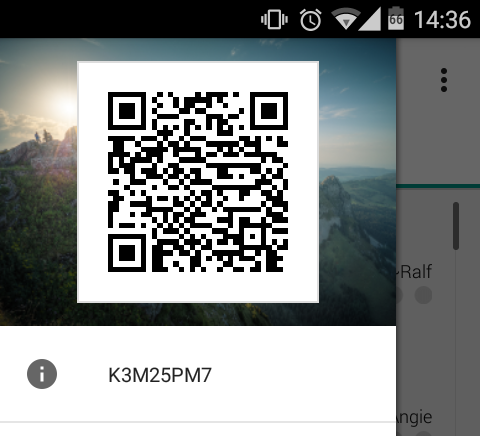
\includegraphics[width=0.6\textwidth]{figures/Threema_ID.png}
\end{frame}

\begin{frame}
  \frametitle{Perfect Forward Secrecy}
  Problem:
  \begin{itemize}
    \item Was passiert wenn der Schlüssel geklaut wird?
    \pause
    \item $\rightarrow$ Alle Nachrichten können entschlüsselt werden
    \item $\rightarrow$ Auch alte Nachrichten, die der Angreifer gespeichert hat
  \end{itemize}
  \pause
  Lösung:
  \begin{itemize}
    \item Sitzungsschlüssel (Analogie: Suppe)
  \end{itemize}
  \center \inputSVG[\def\svgscale{0.2}]{DH_soup}\let\thefootnote\relax\footnote{Bilder von Flicker users jking89 (Joe King), jeffreyww}
\end{frame}

\begin{frame}
  \frametitle{Messaging App Scorecard der \textbf{E}lectronic \textbf{F}rontier \textbf{F}oundation (EFF)}
  \framesubtitle{Auszug aus \url{https://www.eff.org/secure-messaging-scorecard}}
  \center
  \tiny

  \newcommand{\myMarkSize}{0.5cm}
  \newcommand{\myCheck}{
\includegraphics[width=\myMarkSize]{eff_check}}
  \newcommand{\myCross}{
\includegraphics[width=\myMarkSize]{eff_cross}}
  \Wider[4.5em]{
  \begin{tabular}{@{} m{1.8cm}@{\hspace{1mm}} >{\centering\arraybackslash}m{1.7cm}@{\hspace{1mm}} >{\centering\arraybackslash}m{1.5cm}@{\hspace{1mm}} >{\centering\arraybackslash}m{1.2cm}@{\hspace{1mm}} >{\centering\arraybackslash}m{1.9cm}@{\hspace{1mm}} >{\centering\arraybackslash}m{1.0cm}@{\hspace{1mm}} >{\centering\arraybackslash}m{1.37cm}@{\hspace{1mm}} >{\centering\arraybackslash}m{0.6cm}@{\hspace{1mm}} @{}}
    \toprule \\
     & Transportweg\-verschlüs\-selung & Ende-zu-Ende verschlüsselt & Iden\-ti\-täts\-prü\-fung & Perfect Forward Secrecy & Open Source & Sicherheits\-konzept dokumentiert & Audit \\
    \midrule \\
    Facebook chat 	& \myCheck & \myCross & \myCross & \myCross & \myCross & \myCross & \myCheck \\
    Google Hangouts 	& \myCheck & \myCross & \myCross & \myCross & \myCross & \myCross & \myCheck \\
    iMessage 		& \myCheck & \myCheck & \myCross & \myCheck & \myCross & \myCheck & \myCheck \\
    Skype 		& \myCheck & \myCross & \myCross & \myCross & \myCross & \myCross & \myCross \\
    Whatsapp 		& \myCheck & \myCross & \myCross & \myCross & \myCross & \myCross & \myCheck \\
    Threema 		& \myCheck & \myCheck & \myCheck & \myCheck & \myCross & \myCheck & \myCross \\
    Textsecure		& \myCheck & \myCheck & \myCheck & \myCheck & \myCheck & \myCheck & \myCheck \\
    \bottomrule
  \end{tabular}}

\end{frame}

\section{E-Mail Verschlüsselung}

\frame{%
  \frametitle{Inhaltsverzeichnis}
  \tableofcontents[currentsection]
}

\begin{frame}
  \frametitle{PGP}
  \begin{columns}[c]
    \begin{column}{0.5\textwidth}
      \begin{itemize}
	\item \textbf{P}retty \textbf{G}ood \textbf{P}rivacy
        \item OpenPGP als offener Standard
        \item Phil Zimmermann (1991)
        \item Ver- und Entschlüsselung
        \item Digitale Signatur
      \end{itemize}
    \end{column}
    \begin{column}{0.5\textwidth}
          Integration in E-Mail Client
        \begin{itemize}
          \item Thunderbird: Enigmail
          \item Mail: GPGTools
          \item Outlook: ---
        \end{itemize}
    \end{column}
  \end{columns}

\end{frame}

\begin{frame}
  \frametitle{PGP}
  \center
   Thunderbird\\[0.2em]
   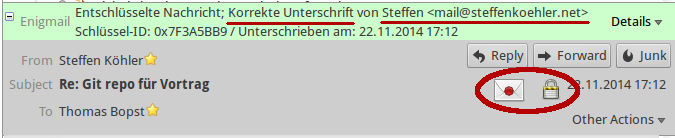
\includegraphics[width=\textwidth]{Enigmail-Screenshot}\\[0.7em]
   Apple Mail\\[0.2em]
   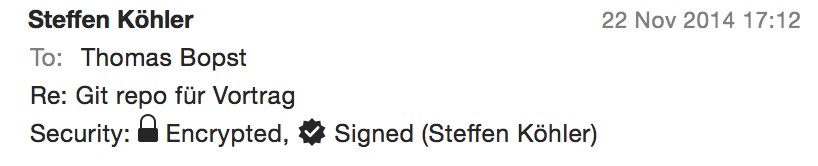
\includegraphics[width=\textwidth]{AppleMail-Screenshot}
\end{frame}

\begin{frame}
  \frametitle{Schlüsselserver (Keyserver)}
  \begin{columns}[c]
    \begin{column}{0.5\textwidth}
      \begin{itemize}
       \item Schlüssel können nicht gelöscht werden
       \item Schlüssel können wiederrufen werden
      \end{itemize}

    \end{column}
    \begin{column}{0.5\textwidth}
      \center \inputSVG[\def\svgscale{0.15}]{Orange_blue_keyserver_de}
    \end{column}
  \end{columns}
\end{frame}

\begin{frame}
  \frametitle{Identitätsprüfung}
  \begin{itemize}
    \item Keine Echtheitsgarantie für Schlüssel auf Schlüsselserver
    \item ``Web of Trust''
    \note{Schlüssel nur signieren wenn WIRKLICH geprüft}
  \end{itemize}
  \center \inputSVG[\def\svgscale{0.2}]{Orange_blue_web_of_trust_de}
\end{frame}

\begin{frame}
  \frametitle{Signierte E-Mail}
  \begin{columns}[c]
    \begin{column}{0.5\textwidth}
      \begin{itemize}
	\item Garantiert Echtheit des Absenders
	\item Ermöglicht Detektion von Manipulationen
	\item Keine Verschlüsselung!
	\note{Unterschriebener Vertrag}
	\item Kann aber mit Verschlüsselung kombiniert werden
      \end{itemize}
    \end{column}
    \begin{column}{0.5\textwidth}
      \center \inputSVG[\def\svgscale{0.2}]{Orange_blue_digital_signature_de}
    \end{column}
  \end{columns}
\end{frame}

\begin{frame}
  \frametitle{Wie kann ich E-Mail Verschlüsselung verwenden?}

      Konfiguration:
      \begin{enumerate}
        \item Schlüsselpaar generieren
        \item Widerrufszertifikat erzeugen
        \item Öffentlichen Schlüssel auf Schlüsselserver laden
        \item Öffentliche Schlüssel von Bekannten herunterladen
      \end{enumerate}

\end{frame}

\section{Fazit}

\frame{%
  \frametitle{Inhaltsverzeichnis}
  \tableofcontents[currentsection]
}

\begin{frame}
  \frametitle{Generelle Tips}
  \begin{itemize}
   \item Regelmäßige Updates
   \item Gesundes Maß an Misstrauen
   \item Sich überlegen wem man welche Daten anvertrauen möchte (z.B. Payback-Karten, Profile)
   \item Wie finanziert sich ein kommerzielles Unternehmen über kostenlose Dienste?
   \item Werden meine Daten an Dritte weitergegeben?
   \item Das Internet vergisst nichts!
  \end{itemize}
\end{frame}

\begin{frame}
  Deine Spuren im Netz
  \frametitle{Zusammenfassung}
  \begin{itemize}
   \item Exzessive Profilbildung
  \end{itemize}

  Instant Messaging
  \begin{itemize}
   \item Sicherheit vor Ausspähen bietet nur Verschlüsselung
   \item Die Wahl der richtigen App
  \end{itemize}

  E-Mail Verschlüsselung
  \begin{itemize}
   \item PGP-Integration für Thunderbird und Apple Mail
   \item Digitale Signatur
  \end{itemize}

\end{frame}


\frame{\emph{Lasst euch nicht überwachen und verschlüsselt immer schön eure Kommunikation ;-)}}

\end{document}
